\documentclass{article}[18pt]
\usepackage{../../../../format}
\lhead{Algorithms and Data Structures - Matthew Johnson}
\lstset{language=Python,
    basicstyle=\ttfamily,
    keywordstyle=\bfseries,
    showstringspaces=false,
    morekeywords={if, else, then, print, end, for, do, while, Input, Output},
    tabsize=4
}
\usepackage{tabularx}
\begin{document}
\begin{center}
\underline{\huge Arrays and Lists}
\end{center}
\section{Arrays}
\textbf{Array} - A sequence of elements $a_1, a_2 ... a_n$\\
\\
An array is usually denoted something like:\\
\texttt{A[1],A[2],...,A[n]} or \texttt{A[1...n]}\\
\\
They're usually in consecutive memory cells, but we (usually) don't care where exactly.\\
\\
All array elements are of the same time, e.g. integer. Can declare as \texttt{integer A[1...n]}\\
\\
\begin{tabular}{lllllll}
Index&0&1&2&3&4&5\\ \cline{2-7} 
\multicolumn{1}{l|}{Variable}&\multicolumn{1}{l|}{H}& \multicolumn{1}{l|}{e}& \multicolumn{1}{l|}{l}& \multicolumn{1}{l|}{l}& \multicolumn{1}{l|}{o}&\multicolumn{1}{l|}{\textbackslash 0} \\ \cline{2-7} 
&&&&&&\\ \cline{2-7} 
\multicolumn{1}{l|}{Address}&\multicolumn{1}{l|}{0x23451}&\multicolumn{1}{l|}{0x23452}&\multicolumn{1}{l|}{0x23453}&\multicolumn{1}{l|}{0x23454}&\multicolumn{1}{l|}{0x23455}&\multicolumn{1}{l|}{0x23456}\\ \cline{2-7} 
\end{tabular}
\subsection{Questions}
\textit{How do we find the ith element, how long does it take?}\\
Go to address and read the data, a quick operation. Not affected by how large the data structure is\\
\\
\textit{What if we want to erase an element?}\\
Once again, easy to find element. However there would be an empty space left, so all following elements would have to be shifted, making it a slow process overall. Affected by size of dataset and position in the dataset.\\
\\
\textit{The size of an array is fixed when we declare it. How big should we make it?}\\
Could make it very big so you don't run out, but this is a waste of allocated memory. In practice make it correct size, then if size needs to be increased, add a pointer to a different bit of memory, but this adds complexity.
\section{Linked lists}
\begin{itemize}
\item A \textbf{list} is made up of \textbf{nodes}. Each node stores an element (a piece of data) plus a pointer or "\textbf{link}" to another node
\item The first node is called the \textbf{head}
\item The last node, called the \textbf{tail} points to null
\item The nodes may be scattered all over the memory
\item Each node points to the next node in the list
\end{itemize}
\subsection{Implementing a list}
Assume for a list \texttt{L} we have pointers to the first as well as the last node of list:
\begin{itemize}
\item \texttt{L.head}
\item \texttt{L.tail}
\item (and possibly we also have \texttt{L.size}) - if the size of the list is often requested, it is easier to set this up at the start, rather than calculating every time
\end{itemize}
May refer to node \texttt{N} using:
\begin{itemize}
\item \texttt{N.data}, the element
\item \texttt{N.next}, the link, the next node in the list (may be \texttt{NULL})
\end{itemize}
\texttt{NULL} means "there's nothing there", i.e., last element has no successor
\subsection{A linked list}
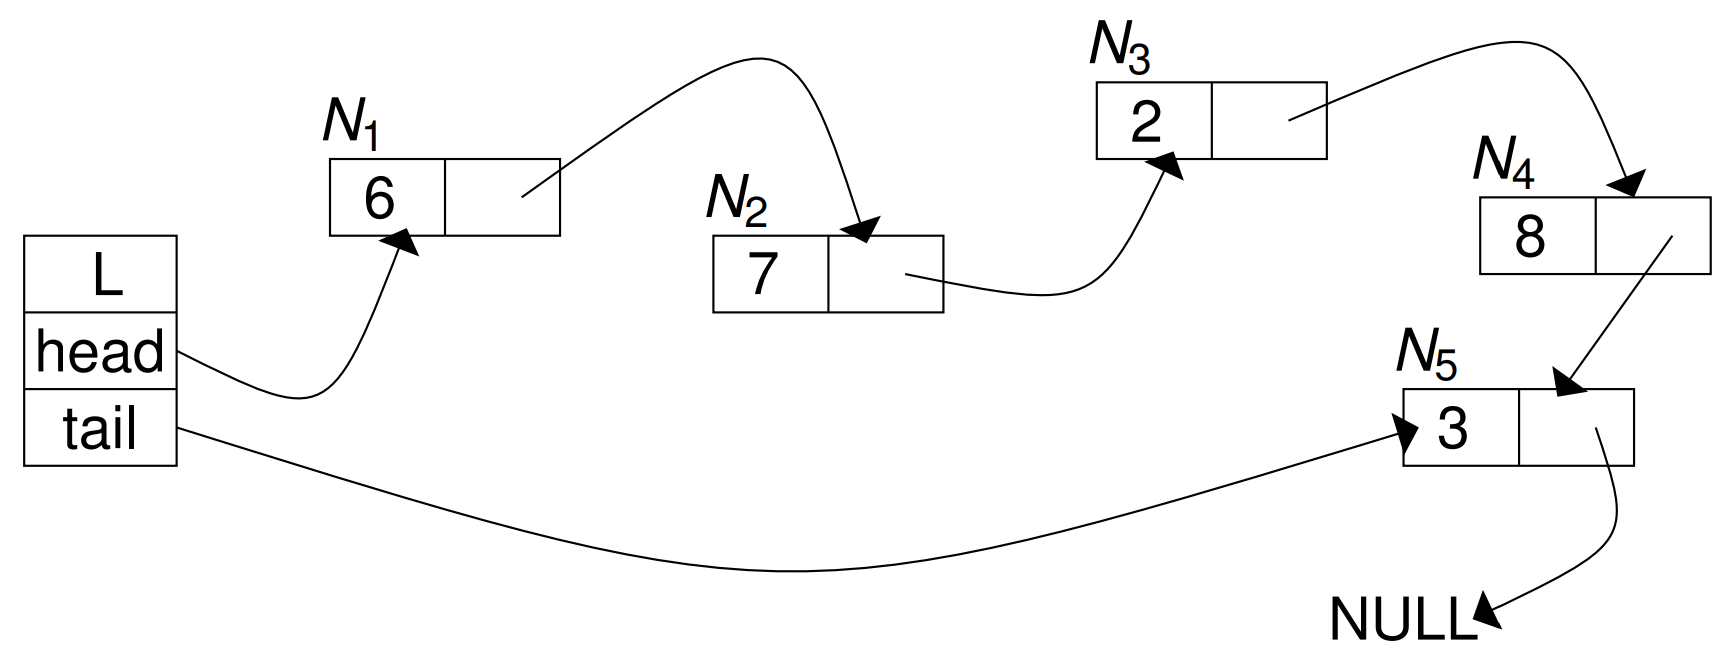
\includegraphics[width=10cm]{Linked_List.png}
\subsection{Finding the ith item}
How would we like \texttt{L.find(i)} to find the \textit{i}th piece of data in a list? How can we do this? How long will it take?\\
\\
Input:list L\\
Output: \textit{i}th item in L\\
\begin{lstlisting}[mathescape=true]
#Checks i is in the list
if i>l.size then
	return error
end if

#Stops error you would get if i was 1
if i=1 then 
	return l.head.data
end if

#Walk through the list
current_node=l.head
for j = 2 to i do
	current_node=current_node.next
return current_node.data
\end{lstlisting}
Need to follow all pointers until you come to the correct piece of data, unlike an array.
\subsection{Altering the list}
How can we alter the list? Anything that inserts or removed must fix all references to predecessors and successors\\
\textbf{Deletion of the head}\\
Input: List L\\
Output: List L with head deleted\\
\begin{lstlisting}[mathescape=true]
# If list is empty then return an error
if l.head=NULL then
	return error
end if

# If list only has one element, set the tail as null
if l.head=l.tail then
	l.tail=NULL
end if

# Set the next element as the head
l.head=l.head.next
\end{lstlisting}


\textbf{Insertion of v after N}\\
Input: list L, data v, node N\\
Output: L with v inserted after N
\begin{lstlisting}[mathescape=true]
node M
M.data=v
# incorrect if N is the last object
if L.tail=N
	L.tail=M

N.next=M
M.next=N.next
\end{lstlisting}
\section{Arrays vs Lists}
\begin{tabularx}{\textwidth}{X|X|X}
                    & Array & Linked List \\ \hline
Data Access        
&
Fast
&
Slow

\\ \hline
Insertion, deletion 
&
Slow
&   
Fast
         
\end{tabularx}
\section{Doubly linked lists}
\begin{itemize}
\item A node in  a \textbf{doubly} linked list stores two references:
\begin{itemize}
\item a next link, which points to the next node in the list
\item a prev link, which points to the previous node in the list
\end{itemize}

\item To simplify, we add two \textbf{dummy} or sentinel nodes at the ends of the doubly linked list:
\begin{itemize}
\item The header has a valid next reference but a null prev reference
\item The trailer has a valid prev reference but a null next reference
\item These act as the head and tail of the list, contain no data
\item These are useful as they will never be deleted during operations on the list.
\end{itemize}
\end{itemize}

A doubly linked list needs to store references to the two sentinel nodes and a size counter keeping track of the number of nodes in the list (not counting sentinels)\\
\\
An empty list would have the two sentinel nodes pointing to each other
\section{Circularly linked list}
\begin{itemize}
\item A \textbf{circularly} linked list has the same kind of nodes as a singly linked list. That is, each node has a next pointer and a reference to an element
\item The circularly linked list has no beginning or end. You can think of it as a singly linked list, where the last nodes next pointer, instead of being \texttt{NULL}, points back to the first node
\item Instead of references to the head and tail, we mark a node of a circularly linked list as the cursor. The cursor is the starting node when we traverse the list
\end{itemize}
\textbf{Deletion from a doubly linked list}
Input: List L, Node N\\
Output: L with N removed\\
\newpage
\begin{lstlisting}[mathescape=true]
M=N.prev
P=N.next
M.next=P
P.prev=M
N.prev=NULL
N.next=NULL
L.size=L.size-1
\end{lstlisting}


\section{Question about an array}
\begin{lstlisting}[mathescape=true]
Input: n numbers in array A[0],. . .,A[n-1]
Output: ?
	for i=0 to n-2 do
		e = A[i]
		p = i
		for j=i+1 to n-1 do
			if A[j]<e then
				e = A[j]
				p= j
			end if
		end for
		swap A[i] and A[p]
	end for
	return A
\end{lstlisting}
What is the output and how is obtained. How long does this procedure take (that is, say, how many times do we make the comparison of A[j] and e in the condition of the \textbf{if} statement\\
\begin{itemize}
\item First time through the loop, puts the smallest item in the array in A[0]
\item Then puts the second smallest item in the array in A[1] etc etc
\item This provides a list sorted from smallest to largest
\item This is running the sorting algorithm selection sort
\item Comparisons (n-1)+(n-2)...
\item Complexity is approximately $n^2$
\end{itemize}
\end{document}